\iflanguage{english}
{\chapter{Grundlagen}}
{\chapter{Background}}
\label{sec:background}


This background chapter provides the essential concepts necessary for understanding the key techniques, models, and algorithms in this thesis. It covers the fundamentals of High-Resolution Human Texture Estimation(HRHumanTex), including uv texture mapping~\cite{10.1145/566654.566590}, deep learning method for super-resolution(SR), diffusion models~\cite{rombach2021highresolution} and DreamBooth~\cite{ruiz2023dreamboothfinetuningtexttoimage} fine-tuning.

\section{3D Human Reconstruction}

In recent years, there has been remarkable progress in reconstructing realistic 3D human bodies, driven by growing demands in area such as film production, virtual try-on(VTO), and human-computer interaction applications. These method attempt to estimate detailed 3D geometry and appearance from monocular or multi-view images or videos, with growing attention to texture fidelity and lifelike pose representation. Existing 3D human body reconstruction methods can be broadly categorized into explicit and implicit approaches.
Explicit methods often rely on parametric models like SMPL~\cite{SMPL:2015}, while implicit methods use volumetric or neural field representations~\cite{mildenhall2020nerf}.


\section{Explicit Parametric Human Models}

Parametric human body models represent the 3D surface of the human body using low-dimensional shape and pose parameters. The most widely used model is the Skinned Multi-Person Linear (SMPL) model~\cite{SMPL:2015}.

\subsection{SMPL Model}

The SMPL model defines a function that generates a 3D mesh of a human body with \( N = 6890 \) vertices, controlled by parameters that represent body shape and pose:

\[
\mathcal{M}(\boldsymbol{\beta}, \boldsymbol{\theta}) = W(T(\boldsymbol{\beta}, \boldsymbol{\theta}), J(\boldsymbol{\beta}), \boldsymbol{\theta}, \mathcal{W})
\]

Where:

 \( \boldsymbol{\beta} \in \mathbb{R}^{10} \): Shape parameters controlling identity, typically obtained via Principal component analysis(PCA).
 
 \( \boldsymbol{\theta} \in \mathbb{R}^{72} \): encode joint rotations in axis-angle format.
 
 \( T(\cdot) \): produces a deformed template mesh based on shape and pose.
 
 \( W(\cdot) \): a linear blend skinning function
 
 \( J(\boldsymbol{\beta}) \): Joint locations
 
 \( \mathcal{W} \): Blend weights

SMPL is popular because of its smooth surface modeling and ease of integration into learning-based pipelines and modern graphics engines. Figure \ref{fig:SMPL} shows how SMPL represents human body shapes.

\subsection{SMPL-X Extension}

SMPL-X~\cite{SMPL-X:2019} extends the original SMPL by including expressive face modeling, articulated hands, and a richer set of body pose parameters. Specifically, it adds facial expression blendshapes and hand pose parameters (15 joints per hand) to better capture complex gestures. This makes SMPL-X better in application scenarios such as requiring full-body expressiveness and emotional rendering.

\begin{figure}[ht]
	\centering
	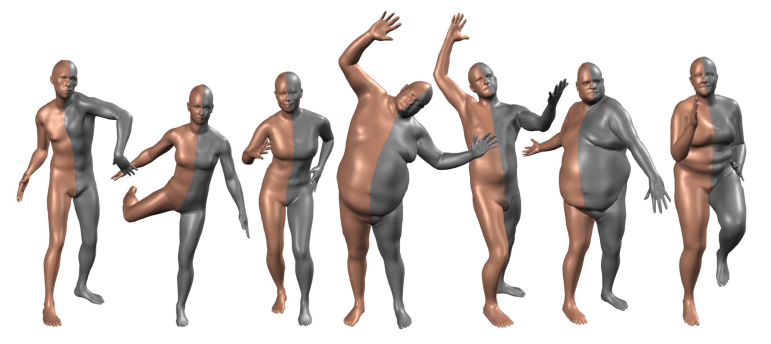
\includegraphics[width=1\textwidth]{fig/smpl.png}
	\caption{A Skinned Multi-Person Linear Model,SMPL \cite{SMPL:2015}}
	\label{fig:SMPL}
\end{figure}

\subsection{UV Texture Space}

In computer graphics, a UV texture map~\cite{10.1145/566654.566590} is a 2D representation of a 3D surface; it is a standard technique for projecting 3D surface  textures into 2D image space. The SMPL model~\cite{SMPL:2015} includes a predefined UV layout that flattens the surface of a 3D body surface onto a 2D texture coordinate system. Each vertex on the 3D body is assigned a UV coordinate \((u,v) \in [0,1]^2\), allowing per-vertex appearance to be stored as an image; figure~\ref{fig:uv-layout} shows a standard SMPL UV layout.

\begin{figure}[h]
    \centering
    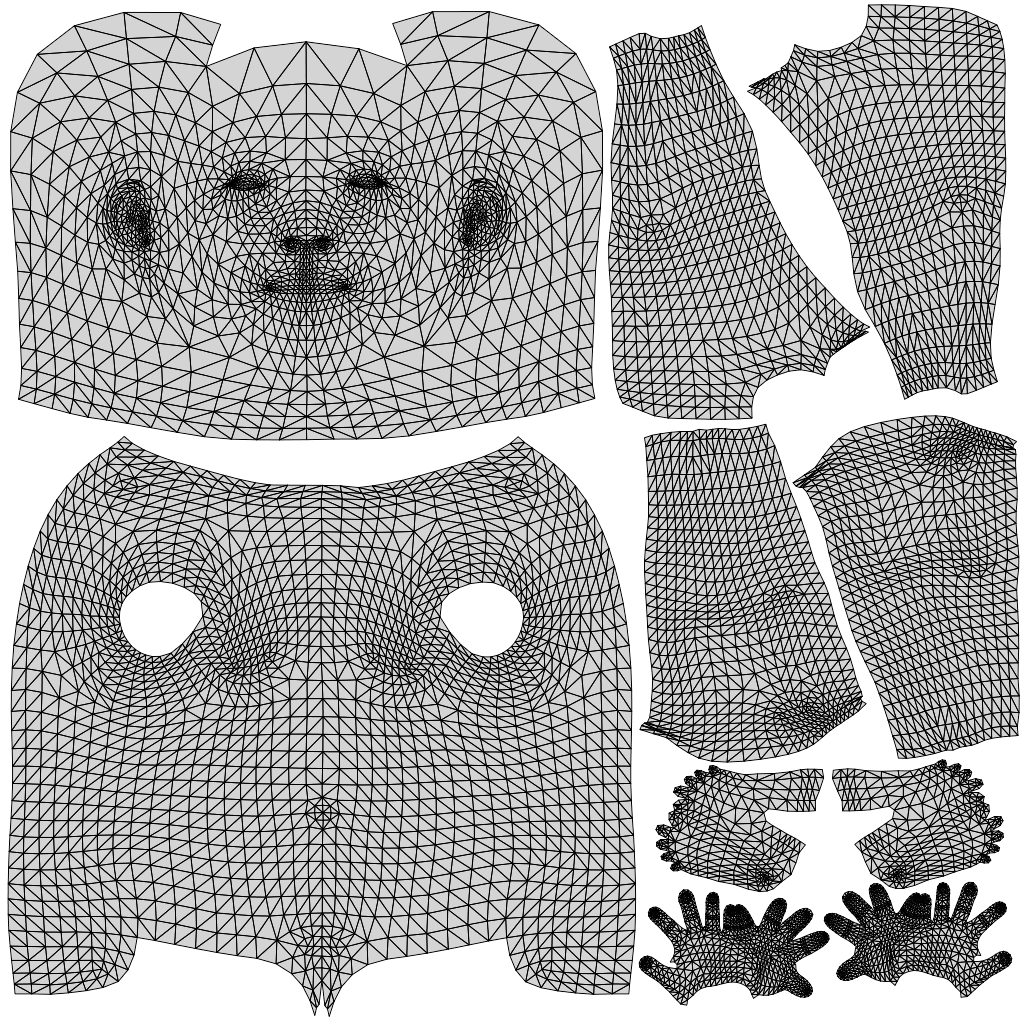
\includegraphics[width=0.45\textwidth]{fig/smpl_uv_20200910.png}
    \caption{SMPL UV layout. Each body part is mapped to a distinct region in the UV space.~\cite{SMPL:2015}}
    \label{fig:uv-layout}
\end{figure}

\subsection{Partial Texture Estimation}

Given a single image as input, only the visible surface can be captured. A texture map can be partially transferred from image pixels to the corresponding UV coordinates using a pixel-to-surface mechanism~\cite{wu2019detectron2} with a segmentation method~\cite{chen2022sghm}. This partial texture calculation will be later introduced in chapter related work and chapter implementation, because I also integrate this partial texture calculation mechanism in my HRHumanTex pipeline. 

\begin{figure}[h]
    \centering
    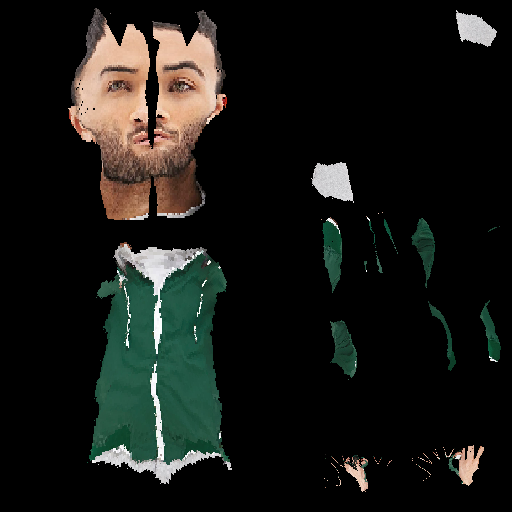
\includegraphics[width=0.4\textwidth]{fig/partial_uv.png}
    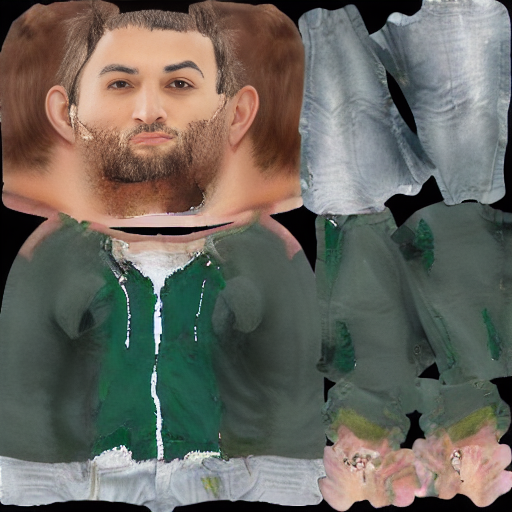
\includegraphics[width=0.4\textwidth]{fig/full_uv.png}
    \caption{Example of a partial UV map estimated from a single view and full texture after inpainting.}
    \label{fig:uv-example}
\end{figure}

\subsection{Full Texture Inpainting}

Since only a part of the surface is observed, completing the partial texture to a full texture could be seen as an inpainting process. The goal is to synthesize plausible appearances for the unobserved regions (e.g., the back of the body, the side of the body), guided by visible information. This task is particularly challenging in high-resolution settings, where global consistency and fine details must be preserved. Figure~\ref{fig:uv-example} shows partial texture and full texture after inpainting.

My thesis focuses on enhancing this inpainting process by leveraging super-resolution and texture learning from high-resolution data.

\section{Super-Resolution (SR) Models}

Super-resolution refers to the process of enhancing image resolution and restoring fine visual details from low-resolution inputs. In this thesis, SR is applied as a key step to upscale 512×512 UV texture maps (produced by SMPLitex~\cite{casas2023smplitex}) to high-resolution (1024×1024) textures, making them suitable for downstream training and inpainting tasks. SR algorithms can broadly be classified into the following categories:

\paragraph{Interpolation-based Methods.}
Bicubic~\cite{1163711}: One of the earliest and simplest methods that rely on mathematical interpolation. Bicubic provides fast but relatively low-quality results with blurring and artifacts and lacks sharp, high-frequency details.

Let \( I_{\text{LR}}(x, y) \) the low-resolution image be the input, and let \( I_{\text{HR}}(u, v) \) the high-resolution output at floating-point coordinates \( (u, v) \) by performing a weighted sum of surrounding pixels in the low-resolution image. The bicubic interpolation computation process could be presented as:

\begin{equation}
I_{\text{HR}}(u, v) = \sum_{i=-1}^{2} \sum_{j=-1}^{2} w(i,j) \cdot I_{\text{LR}}(x+i, y+j),
\end{equation}

where \( x = \lfloor u \rfloor \), \( y = \lfloor v \rfloor \), and the weights \( w(i,j) \) are defined as:

\begin{equation}
w(i,j) = h(u - x - i) \cdot h(v - y - j),
\end{equation}

with \( h(s) \) being the bicubic kernel, commonly implemented as:

\begin{equation}
h(s) = 
\begin{cases}
(1.5)|s|^3 - 2.5|s|^2 + 1, & 0 \leq |s| < 1 \\
-0.5|s|^3 + 2.5|s|^2 - 4|s| + 2, & 1 \leq |s| < 2 \\
0, & \text{otherwise}
\end{cases}
\end{equation}

This cubic kernel is derived from Keys' interpolation method~\cite{1163711}, with the parameter \( a = -0.5 \), offers a smooth approximation but struggles to reconstruct fine texture, which motivates the use of learning-based SR techniques.

\paragraph{\ac{CNN}-based Methods.}
RCAN~\cite{zhang2018rcan}: The Residual Channel Attention Network (RCAN) is a deep CNN-based model designed for high-accuracy SR tasks. It introduces a residual-in-residual (RIR) structure, composed of residual groups (RGs) with both short- and long-skip connections. This architecture enables efficient training of very deep networks (over 400 layers), ensuring stable optimization and preserving low-frequency content information throughout the network. RCAN also integrates a Channel Attention (CA) mechanism, which adaptively rescales channel-wise features, improving its ability to focus on information-rich features and enhance fine visual details in the output. Figure~\ref{fig:rcan} shows the network architecture of RCAN.
\begin{figure}[h]
    \centering
    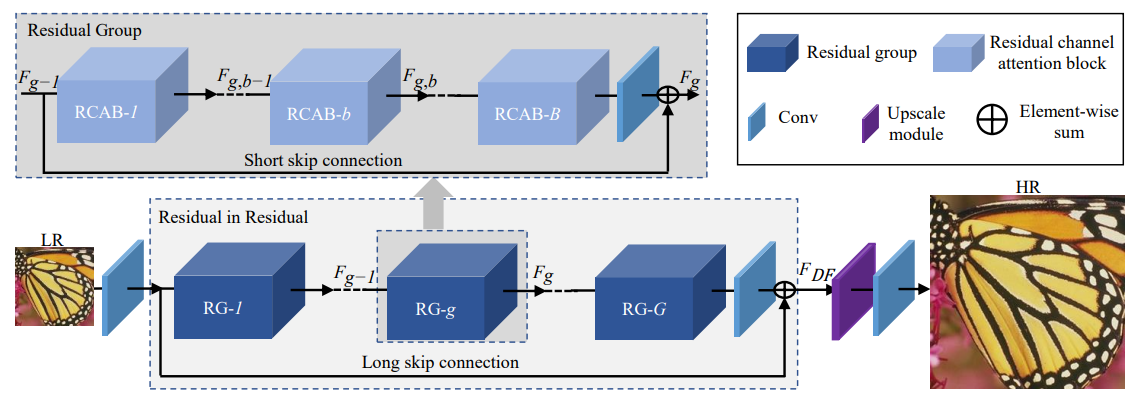
\includegraphics[width=0.95\textwidth]{fig/RCAN.png}
    \caption{Network architecture of residual channel attention network (RCAN).~\cite{zhang2018rcan}}
    \label{fig:rcan}
\end{figure}

\paragraph{\ac{GAN}-based Methods.}
Generative Adversarial Networks~\cite{goodfellow2014generativeadversarialnetworks} have also been successfully applied to super-resolution tasks.
RealESRGAN~\cite{wang2021realesrgan} and BSRGAN~\cite{zhang2021designing}are two representative models in this category. Real-ESRGAN \ref{fig:realesrgan} extends ESRGAN~\cite{wang2018esrgan} to better handle complex, real-world degradations by introducing a high-order degradation model that simulates multiple degradation processes, such as blur, various types of noise, and compression artifacts. Figure~\ref{fig:realesrgan} shows its architecture. BSRGAN takes a similar direction, introducing a robust degradation pipeline that randomly combines diverse degradation operations and their orders, creating a more challenging training setup that enhances robustness to unseen artifacts.
\begin{figure}[h]
    \centering
    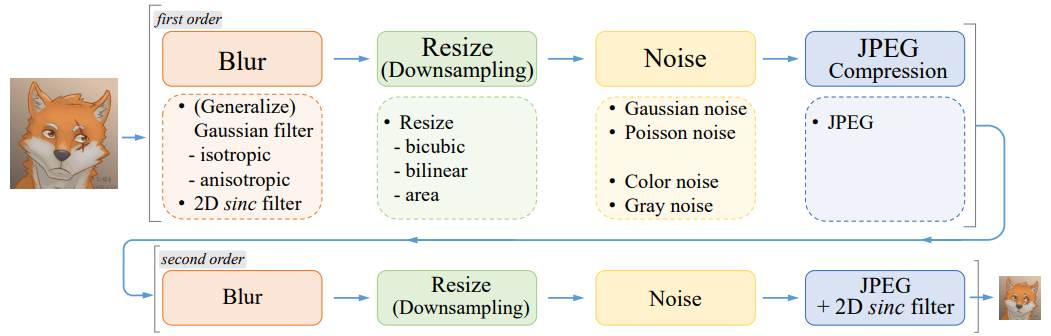
\includegraphics[width=0.95\textwidth]{fig/RealESRGAN.png}
    \caption{Real-ESRGAN Architecture.~\cite{wang2021realesrgan}}
    \label{fig:realesrgan}
\end{figure}

\paragraph{Transformer-based Methods.}
With the success of Transformers in vision tasks, models like
SwinIR~\cite{liang2021swinir} and SRFormer~\cite{zhou2023srformer} have emerged as strong alternatives to \ac{CNN}. SwinIR built on Swin Transformer~\cite{liu2021swintransformerhierarchicalvision}. It combines local attention with shifted window mechanisms to efficiently model both short- and long-range dependencies. The architecture consists of shallow feature extraction, deep feature extraction via Residual Swin Transformer Blocks (RSTB), and reconstruction. SRFormer improves upon SwinIR by introducing Permuted Self-Attention (PSA), which allows larger attention windows(e.g., \(24 \times 24\)) with reduced computational cost. Instead of scaling the feature dimensions, PSA encodes spatial information into the channel space. In addition, SRFormer uses a convolution-enhanced feed-forward network (ConvFFN) to better capture and reconstruct high-frequency image content. Figure~\ref{fig:srformer} shows the overrall architecture of SRFormer.

\begin{figure}[h]
    \centering
    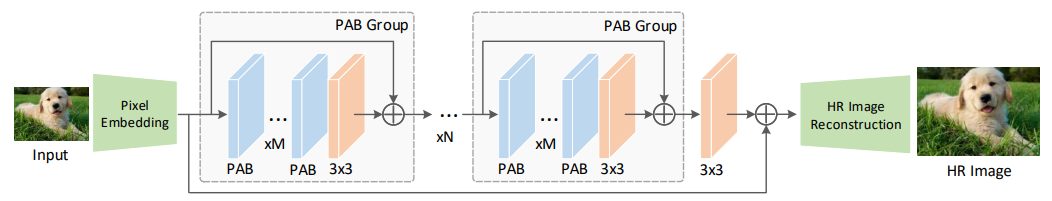
\includegraphics[width=0.95\textwidth]{fig/SRFormer.png}
    \caption{Overall architecture of SRFormer.~\cite{zhou2023srformer}}
    \label{fig:srformer}
\end{figure}

\paragraph{Diffusion-based Methods.}
Recent improvements in generative artificial intelligence have also introduced diffusion-based approaches for super-resolution tasks.
DiffBIR~\cite{lin2024diffbir} and StableSR~\cite{wang2024exploiting} represents this line of research. DiffBIR addresses Blind Image Restoration (BIR) by proposing it in two stages: (1) degradation removal using a learned predictor and (2) synthesizing the high-resolution content with a latent diffusion model~\cite{rombach2021highresolution}. It employs IRControlNet to guide image synthesis with fidelity-aware conditioning. A region-adaptive guidance mechanism helps balance realism and detail, especially in high-variance regions. Figure~\ref{fig:diffbir} shows the two stage pipeline of DiffBIR. StableSR, in contrast, leverages frozen, pre-trained diffusion models for SR, avoiding the need to retrain the entire model for each task. It introduces a lightweight time-aware encoder that adaptively modulates features across diffusion steps and a controllable feature wrapping (CFW) module to refine outputs during decoding. The model also adopts a progressive aggregation sampling strategy that ensures boundary continuity for large-resolution outputs. 

\begin{figure}[h]
    \centering
    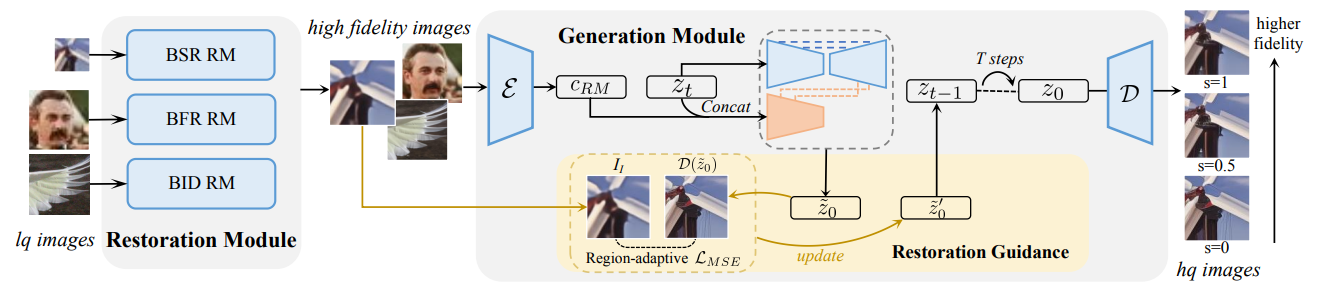
\includegraphics[width=0.95\textwidth]{fig/DiffBIR.png}
    \caption{The two-stage pipeline of DiffBIR.~\cite{lin2024diffbir}}
    \label{fig:diffbir}
\end{figure}

Each super-resolution approach has distinct advantages and limitations. In this work, I systematically compare representative models from each category to identify the most effective method for UV texture upscaling. The SR evaluation considers PSNR, LPIPS, SSIM, and FID, aiming to select the optimal SR model to support high-resolution inpainting model training.

\section{Diffusion Models and Stable Diffusion}

Denoising Diffusion Probabilistic Models (DDPMs)~\cite{ho2020denoising} have emerged as one of the most popular and effective frameworks for image synthesis. These models generate data through an iterative denoising process that progressively removes Gaussian noise from a randomly sampled latent variable. The forward process gradually corrupts a clean image $x_0$ over $T$ steps by adding noise according to:

\begin{equation}
q(x_t \mid x_{t-1}) = \mathcal{N}(x_t; \sqrt{\alpha_t} x_{t-1}, (1 - \alpha_t)\mathbf{I})
\end{equation}

This produces a latent variable $x_T$ that approaches an isotropic Gaussian distribution. The generative model is then trained to reverse this process:

\begin{equation}
p_\theta(x_{t-1} \mid x_t) = \mathcal{N}(x_{t-1}; \mu_\theta(x_t, t), \Sigma_\theta(x_t, t))
\end{equation}

In practice, a neural network $\epsilon_\theta$ is trained to predict the added noise using a simplified loss function:

\begin{equation}
\mathcal{L}_{\text{DDPM}} = \mathbb{E}_{x_0, \epsilon, t}\left[ \| \epsilon - \epsilon_\theta(x_t, t) \|_2^2 \right]
\end{equation}

\textbf{Stable Diffusion}~\cite{rombach2022high} improves the efficiency of DDPMs by operating in a learned latent space $z = \mathcal{E}(x)$ using a variational autoencoder (VAE) rather than pixel space, where $x$ is the original image. The denoising process is then performed in the latent space $z$, and the final image is reconstructed via a decoder $x' = \mathcal{D}(z)$. The latent-space diffusion training objective function is defined as follows:

\begin{equation}
\mathcal{L}_{\text{LDM}} = \mathbb{E}_{z_0, \epsilon, t}\left[ \| \epsilon - \epsilon_\theta(z_t, t, c) \|_2^2 \right]
\end{equation}

where $z_t$ is a noisy latent vector, $c$ is an external conditioning signal (such as text, pose, or UV maps), and $\epsilon_\theta$ is typically a UNet~\cite{ronneberger2015unetconvolutionalnetworksbiomedical} model with cross-attention mechanisms to incorporate the conditioning input. Figure~\ref{fig:stablediffusion} show the Stable Diffusion architecture.


\begin{figure}[h]
    \centering
    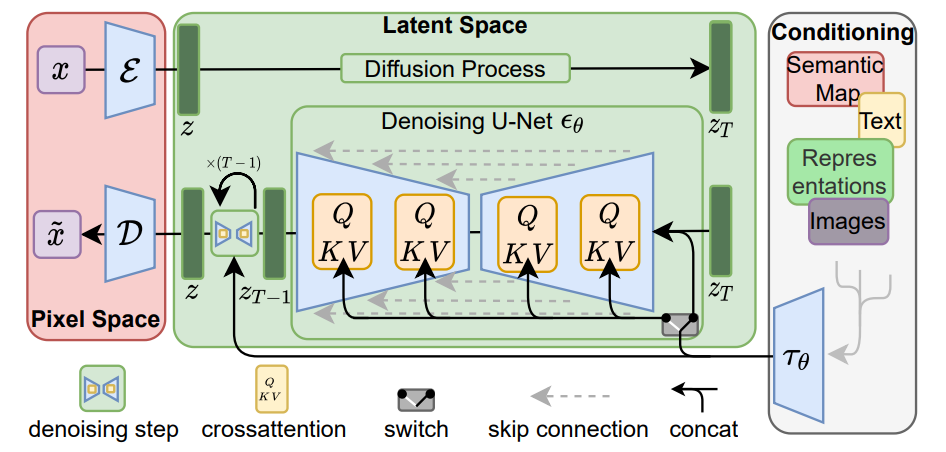
\includegraphics[width=0.95\textwidth]{fig/stablediffusion.png}
    \caption{Stable Diffusion Architecture.~\cite{rombach2021highresolution}}
    \label{fig:stablediffusion}
\end{figure}

In this thesis, Stable Diffusion v1.5 is fine-tuned to perform high-resolution UV texture inpainting, where conditioning is provided by partial UV inputs.

\section{DreamBooth Fine-tuning}

\textbf{DreamBooth}~\cite{ruiz2023dreamboothfinetuningtexttoimage} is a fine-tuning method designed to personalize a pre-trained large-scale text-to-image diffusion model with only a few reference images. It introduces a new identifier token $v^*$ (such as, a photo of $v^*$ person) that is embedded within the text encoder and associated with a specific visual identity. Figure~\ref{fig:dreambooth} shows its fine-tuning pipeline.

\begin{figure}[h]
    \centering
    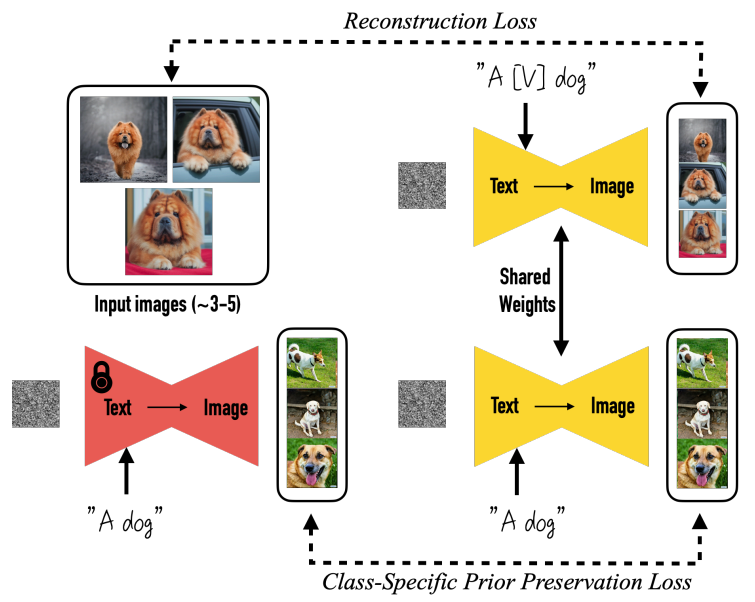
\includegraphics[width=0.65\textwidth]{fig/dreambooth.png}
    \caption{Dreambooth fine-tuning pipeline.~\cite{ruiz2023dreamboothfinetuningtexttoimage}}
    \label{fig:dreambooth}
\end{figure}

The overall fine-tuning objective of DreamBooth can be expressed as a composite objective function:

\begin{equation}
\mathcal{L}_{\text{DreamBooth}} = \lambda_1 \mathcal{L}_{\text{diffusion}} + \lambda_2 \mathcal{L}_{\text{recon}} + \lambda_3 \mathcal{L}_{\text{CLIP}}
\end{equation}

where:
\begin{itemize}
  \item $\mathcal{L}_{\text{diffusion}}$: standard DDPM loss for denoising.
  \item $\mathcal{L}_{\text{recon}}$: reconstruction loss to preserve fine visual details.
  \item $\mathcal{L}_{\text{CLIP}}$: CLIP-based alignment to maintain textual-image consistency.
\end{itemize}

By injecting personalized identity tokens into the text prompt and supervising the generation with both pixel-level and perceptual constraints, DreamBooth effectively captures and reproduce the unique apperance characteristics of a subject, even with limited data. 

In this thesis, DreamBooth is employed to specialize Stable Diffusion for personalized texture inpainting. Specifically, each model is trained on 12 to 266 high-resolution UV texture images associated with a specific clothing/person identity "a sks texturemap." This approach enables the model to fill missing regions in partial UV textures while preserving the semantic consistency and visual quality of the original identity.


